\capitulo{5}{Aspectos relevantes del desarrollo del proyecto}

Este apartado recoge los aspectos más interesantes del desarrollo del proyecto, el ciclo de vida utilizado y los detalles de mayor relevancia de las fases de análisis, diseño e implementación.

\section{Metodologías aplicadas}

Para la realización de este proyecto se ha decidido seguir una metodología ágil siempre que ha sido posible. Por ello, se han seguido ciertas líneas de trabajo. A continuación se listan:

\begin{itemize}
    \item Se ha dividido el desarrollo del proyecto en múltiples \english{sprints}.
    \item Se han ido proponiendo nuevos requisitos y objetivos a medida que se iban cumpliendo los anteriores.
    \item Se han realizado reuniones entre todos los integrantes al acabar cada \english{sprint}.
    \item Al acabar cada \english{sprint} se ha realizado una demostración siempre que los cambios eran sustanciales.
    \item Se han organizado las diferentes tareas y objetivos a completar en un tablero Kanban\footnote{\url{https://kanbantool.com/es/tablero-kanban}}.
    \item Se ha asociado una duración estimada a cada tarea antes de realizarla.
\end{itemize}

\section{Propuesta del proyecto}
La idea de este proyecto nace con el objetivo de crear una herramienta que ayude a obtener y descargar información sobre una familia de productos concreta de la web de compras por internet \english{Amazon.com} con el objetivo de hacer múltiples estudios sobre los diferentes conjuntos de datos obtenidos.

Desde un primer momento se ha querido obtener la mayor cantidad de campos de información, es por ello que una vez el proceso ha sido completado, obtenemos la siguiente información de cada producto:

\begin{description}
    \item[ASIN:] Código identificativo de cada producto.
    \item[Sexo:] Sexo al que va dirigido cada artículo.
    \item[Rango de precios:] El precio de cada producto puede variar en función del color o la talla. Este campo recoge el precio máximo y mínimo de cada producto.
    \item[Marca:] El nombre de la marca de cada artículo.
    \item[Descripción:] Texto que el vendedor ha utilizado para describir y dar detalles de cada producto.
    \item[Puntuación:] Media de las puntuaciones que los clientes han votado a cada producto. Va del 0 al 5.
    \item[Número de valoraciones:] Número de clientes que han proporcionado una valoración del producto.
    \item[Comentarios sobre el producto:] Comentarios completos sobre un producto en el que los compradores dejan su opinión. El número de comentarios a extraer debe ser definido al comenzar el proceso.
    \item[URL:] Dirección web de cada producto
    \item[Imágenes:] Conjunto de imágenes asociadas a cada artículo.
    \item[Contenido de la imagen principal:] Este campo describe el contenido de la imagen principal de cada producto en función de si aparece un modelo o no, y si la cara del modelo es visible o no.
\end{description}

La mayoría de estos campos se pueden extraer directamente del código \english{HTML} de la web de cada producto, pero para ciertos casos es necesario procesar antes la información ya extraída y usarla para crear los campos que faltan. Como es el caso del campo que recoge el contenido de la imagen principal.

A continuación se irán presentando y detallando las diferentes fases de las que se compone el proceso de extracción y procesamiento de datos.

\section{Extracción de los datos}

La herramienta utilizada en este proyecto para realizar el \english{web scraping} ha sido Scrapy. Se han barajado otras opciones como BeautifulSoup\footnote{\url{https://www.crummy.com/software/BeautifulSoup/bs4/doc/}} o Selenium\footnote{\url{https://www.seleniumhq.org/}}.

Las principales diferencias y ventajas que lo separan del resto son:
\begin{itemize}
    \item Es más rápido ya que trabaja de forma asíncrona.
    \item Tiene mejor soporte para parseado de HTML.
    \item Soporta caracteres unicode.
    \item Soporta redirecciones HTTP.
    \item Exportación directa de los resultados a JSON, CSV o XML.
    \item Se puede usar junto a otras librerías como urllib\footnote{\url{https://docs.python.org/3/library/urllib.html}} o BeautifulSoup.
\end{itemize}

\subsection{Arquitectura de Scrapy}

En cuanto a la arquitectura de Scrapy, hay que destacar los tres principales bloques que lo conforman:

\begin{description}
    \item[\english{Items}:] Los diferentes elementos o campos a extraer.
    \item[\english{Spiders}:] Clases escritas por el usuario que contienen los diferentes procedimientos para parsear y extraer los \english{items} de uno o varios enlaces. En este caso hemos hecho uso de 3 \english{spiders}: Una para obtener los enlaces a cada artículo, otra para extraer los comentarios, y la última para el resto de campos.
    \item[\english{Pipelines}:] Apartado responsable de procesar los \english{items} una vez han sido extraidos por las \english{spiders}. En este proyecto se han usado para almacenar los campos extraídos en una base de datos.
\end{description}

\FloatBarrier
    \begin{figure}[!h]
    \centering
    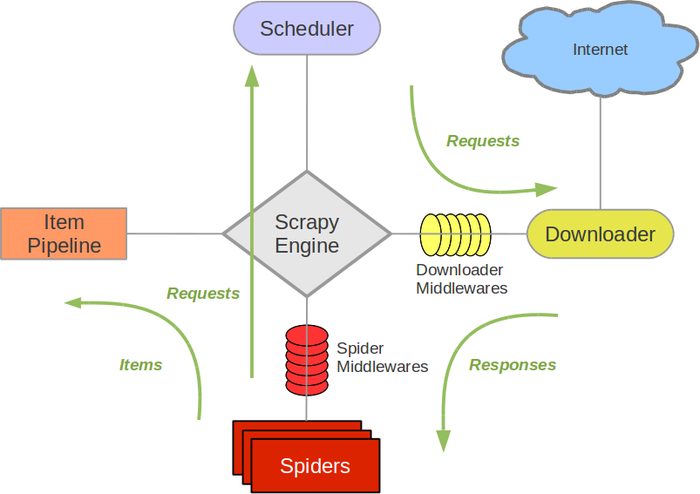
\includegraphics[width=0.8\textwidth]{scrapy_architecture}
    \caption[Arquitectura que sigue Scrapy y sus diferentes componentes]{Arquitectura que sigue Scrapy y sus diferentes componentes.
    \newline
    Imagen extraída de \url{https://doc.scrapy.org/en/0.10.3/topics/architecture.html}}
    \label{fig}
    \end{figure}
\FloatBarrier

\subsection{\english{Spiders} utilizados}
El primer \english{spider} se encarga de extraer los enlaces a los productos. Para ello partimos de la página principal donde se encuentran todos los artículos a extraer. Cabe destacar que no existe un enlace que de acceso a una página web que contenga los productos orientados a ambos sexos, por lo que en caso de querer artículos para hombres y mujeres se necesita una url para cada sexo.

Este \english{spider} además genera un archivo JSON que contiene todos los enlaces que ha extraido. Este archivo será utilizado como punto de partida de los siguientes \english{spiders} para la extracción de los campos de cada artículo.

\imagen{principal-hombres2}{Productos a extraer}

El siguiente \english{spider} es el encargado de extraer la mayoría de campos de un producto. Es necesario destacar los diferentes métodos utilizados para la extracción de estos campos:

\begin{itemize}
    \item Expresiones regulares: El campo del ASIN se extrae directamente del url con ayuda de una expresión regular.
    \item La mayoría de campos se han extraido con la ayuda de expresiones XPath\footnote{\url{https://es.wikipedia.org/wiki/XPath}}, que consisten en parsear el código HTML de la web e identificar el campo que se desea extraer.
    \item Para las imágenes ha sido necesaria la utilización de una librería externa llamada js2xml\footnote{\url{https://github.com/scrapinghub/js2xml}}. Esta librería facilita la extracción de elementos embebidos en código JavaScript usando XPath.
\end{itemize}

\imagen{campos_1}{Posición de algunos de los campos a extraer}

Por último, el tercer \english{spider} del que hacemos uso es el encargado de extraer los comentarios de cada producto. Para ello usamos una expresión XPath sobre una página cuyo url creamos a partir del ASIN de cada artículo.

\imagen{comentarios2}{Comentarios sobre un producto}

En cuanto al \english{pipeline} de nuestro proyecto de Scrapy, cada vez que se extrae un \english{item}, éste es almacenado en una base de datos. El \english{pipeline} se encarga de conectar con la base de datos, crear las tablas necesarias con sus respectivos campos, y cerrar la conexión una vez se han almacenado todos los productos.

\imagen{proyecto_scrapy}{Proceso de \english{web scraping} del proyecto}

\section{Etiquetado manual de las imágenes}

Antes de etiquetar automáticamente las imágenes, es necesario entrenar el clasificador para que éste sea capaz de identificar cada imagen. Para ello se ha tenido que crear un conjunto de datos etiquetado manualmente que sirva de entrenamiento para el clasificador.

Ese conjunto de datos etiquetados o \english{dataset}, se ha generado con la ayuda de la web \english{Dataturks}\footnote{\url{https://dataturks.com}}.

El funcionamiento de esta herramienta es sencillo: basta con crear una lista con los enlaces a las imágenes que se desean etiquetar e indicar las posibles etiquetas que una imagen puede tener. A partir de aquí, la herramienta descarga y muestra secuencialmente todas las imágenes y se ha de decidir que etiqueta corresponde a cada una.

\imagen{dataturks}{Captura de pantalla durante el proceso de etiquetado manual}

Una vez se han etiquetado todas las imágenes, se puede exportar el conjunto de imágenes como un archivo JSON que asocia cada enlace con las etiquetas seleccionadas.

Para este proyecto se han creado dos \english{datasets}. En el primero se diferencian las imágenes en las que aparece un modelo y en las que no, el segundo \english{dataset} parte del anterior e identifica en cuales de las imágenes en las que si hay modelo, a éste se le ve la cara.

\subsection{Problemas encontrados}

El primero de los problemas sufridos relacionados con el etiquetado de imágenes fue precisamente decidir qué etiquetas seleccionar. En un principio la idea era identificar si aparecía un maniquí o no, o incluso si en la imagen no aparecía el producto anunciado. Estas ideas se desecharon ya que había demasiados casos en los que no era demasiado claro qué etiqueta correspondía a cada producto.

Otro problema encontrado ha sido a la hora de identificar si al modelo se le ve la cara o no. Hay muchos casos en los que la cara del modelo está cortada y solo es visible parcialmente. También hay casos en los que el modelo está de espaldas y mirando hacia un lado y solo se intuye la cara de éste. Lo primero que se pensó para estos casos fue un algoritmo que identificase las caras parcialmente, y aunque se han encontrado varios recursos que parecen dar respuesta a este problema, al final se optó por etiquetar las imágenes de forma que si parte de la cara es visible, se clasificaría como que si hay cara.

Algunos de los recursos que se han utilizado para una posible detección parcial de la cara han sido los siquientes:
\begin{itemize}
    \item \english{Partial Face Recognition}: \url{http://www.faceforensics.com/PartialFaceRecog.aspx}
    \item \english{Partial Face Detection in the Mobile Domain}: \url{https://arxiv.org/pdf/1704.02117.pdf}
    \item \english{Dynamic Feature Learning for Partial Face Recognition}: \url{http://openaccess.thecvf.com/content_cvpr_2018/papers/He_Dynamic_Feature_Learning_CVPR_2018_paper.pdf}
    \item \english{A robust face detector under partial occlusion - IEEE Conference Publication}: \url{https://ieeexplore.ieee.org/document/1418825}
    \item \english{Dealing with Inaccurate Face Detection for Automatic Gender Recognition with Partially Occluded Faces}: \url{http://repositori.uji.es/xmlui/bitstream/handle/10234/23941/34130.pdf}
\end{itemize}

\imagen{cara_espalda_parcial}{Ejemplos de modelos con la cara parcialmente visible}

\section{Etiquetado automático de las imágenes}

Para el etiquetado automático de imágenes se ha decidido usar Keras. Existen otros \english{frameworks} que se han tenido en cuenta para este proyecto como pueden ser Pytorch\footnote{\url{https://pytorch.org/}} o Caffe\footnote{\url{https://caffe.berkeleyvision.org/}}, pero se ha usado Keras por varias razones:

\begin{description}
    \item[Experiencia con este \english{framework}:] Ya había trabajado con anterioridad con Keras para clasificación de imágenes.
    \item[Facilidad de uso:] Después de leer e informarme sobre otros \english{frameworks}, Keras me ha parecido el más facil de aprender y de poner en marcha.
    \item[Flexibilidad:] Keras se integra con TensorFlow\footnote{\url{https://www.tensorflow.org/guide/keras}}, es por esto que permite implementar cualquier cosa implemetada con TensorFlow como base.
    \item[Compatibilidad:] Keras es compatible con Google Cloud\footnote{\url{https://cloud.google.com/tpu/}} y Tarjetas gráficas NVIDIA\footnote{\url{https://developer.nvidia.com/deep-learning}}, gracias a ello funciona de forma nativa con Google Colab.
\end{description}

\newpage

\subsection{Validación cruzada}
Para el entrenamiento de estos clasificadores se ha usado la técnica de validación cruzada. Esta técnica consiste en dividir el \english{dataset} en dos conjuntos complementarios y realizar el análisis sobre un subconjunto para luego validarlo con los datos del otro subconjunto. La principal ventaja de este método es que es muy rápido de computar.

Existen variaciones de este método, en el que se suceden varias iteraciones, obteniendo así una mayor precisión. En este caso se ha optado por el método de validación cruzada aleatoria ya que la precisión era aceptable y Keras dispone de una función que facilita este procedimiento \cite{wiki:cruzada}. 

\FloatBarrier
    \begin{figure}[!h]
    \centering
    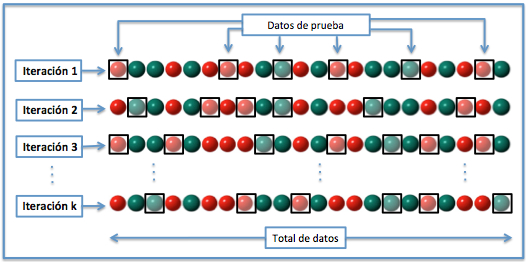
\includegraphics[width=0.9\textwidth]{Random_cross_validation}
    \caption[Validación cruzada aleatoria con $k$ iteraciones]{Validación cruzada aleatoria con $k$ iteraciones. Imagen extraída de \url{https://es.wikipedia.org/wiki/Validacion\_cruzada}}
    \label{fig}
    \end{figure}
\FloatBarrier

Para los clasificadores entrenados en este proyecto, se ha hecho una división del 75\% para el conjunto de entrenamiento y un 25\% para el conjunto de test. En el caso del clasificador que identifica si aparece un modelo o no, se obtiene una precisión de aproximadamente un 93\%. En cambio, para el clasificador que indica si parece la cara del modelo, la precisión es de únicamente un 80\%. La diferencia de precisión entre ambos clasificadores se debe a la complejidad del problema, ya que incluso se han tenido dudas a la hora elegir qué etiquetas usar de forma manual.

\imagen{precision_cara}{Precisión del clasificador Cara/No cara}

El número de iteraciones para el entrenamiento ha sido de 10 para ambos clasificadores. Se ha probado con distintos números de iteraciones pero la precisión obtenida no variaba o decrecía.

\imagen{summary}{Resumen de las capas del clasificador de imágenes}

\subsection{Problemas encontrados}

El principal inconveniente que se ha encontrado en el proceso de clasificación está directamente relacionado con el problema encontrado a la hora de etiquetar las imágenes manualmente. Para el clasificador que identifica si la cara de un modelo es visible, se pensó en utilizar una función de la librería de OpenCV que detecta caras en una imagen con la utilización de \english{Haar Cascades}\footnote{\url{https://docs.opencv.org/3.4.1/d7/d8b/tutorial_py_face_detection.html}}. Los resultados parecían prometedores al principio ya que actúa con una precisión muy alta. Pero el principal problema que se encontró es que no detectaba las caras cortadas. Esto hizo que se desechara la idea y se pasase a entrenar dos clasificadores.

\imagen{opencv_error}{Detección errónea de caras con la librería OpenCV}

\section{Visualización y almacenamiento de todos los productos junto a sus campos}

En este punto, ya tendríamos los clasificadores funcionando y los campos de los productos extraídos. Los pasos siguientes se encargan de satisfacer los objetivos de almacenamiento y visualización de los artículos extraídos:

\begin{enumerate}
    \item Cargar los clasificadores previamente entrenados
    \item Importar todos los productos que se desea clasificar. Esto se hace a partir del archivo JSON que ha generado Dataturks combinado con el archivo JSON creado por Scrapy.
    \item Clasificamos la imagen  principal de cada producto.
    \item Conectamos con la base de datos y creamos una nueva tabla que incluirá las predicciones de cada imagen. Es necesario recordar que la base de datos hasta este momento contiene 3 tablas: Productos, Imágenes y Comentarios. Esta nueva tabla asocia cada predicción con el ASIN del artículo al que pertenece.
\end{enumerate}

Con esto la base de datos quedaría completada. Cabe destacar que se ha elegido crear una nueva tabla en vez de añadir el campo <<predicción>> a una tabla ya existente ya que en un futuro se tendría pensado clasificar mas aspectos de cada artículo como podrían ser los comentarios u otras características de las imágenes.

\subsection{Almacenamiento de los datos}

La base de datos utilizada para almacenar los diferentes productos no es muy compleja. Una vez finalizada la extracción y el procesamiento de los datos, cuenta con 4 tablas con el ASIN de cada artículo como identificador.

\begin{itemize}
    \item La primera tabla, la más general, contiene los diferentes campos de cada producto y el ASIN como clave primaria. Cada entrada pertenece a un artículo diferente.
    \item La tabla de las imágenes almacena los enlaces a cada imagen junto al ASIN del producto al que pertenece. Puede haber varias imágenes para un único producto.
    \item La tabla de los comentarios almacena comentarios asociados a cada artículo. Puede haber varios comentarios de cada producto.
    \item La tabla de predicciones asocia cada artículo con la predicción que el clasificador ha generado para la imagen principal de dicho producto. Cada entrada es de un producto diferente.
\end{itemize}

Por último, es necesario añadir el proceso de creación de un documento Excel a partir de la base de datos ya completada. Para esto se ha utilizado una librería de Python llamada Pandas\footnote{\url{https://pandas.pydata.org/pandas-docs/stable/index.html}}, la cual extrae la información de la base de datos y la exporta a un documento Excel creando una página por cada tabla existente en la base de datos.
\newline

\FloatBarrier
    \begin{figure}[!h]
    \centering
    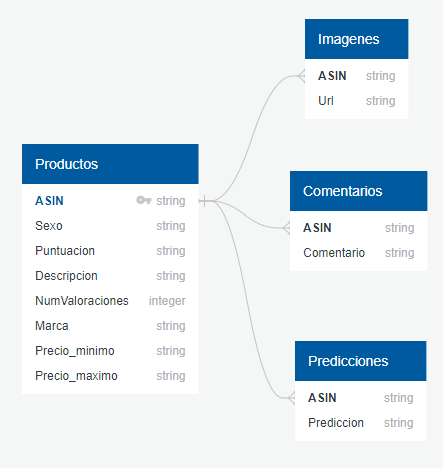
\includegraphics[width=0.8\textwidth]{bd_diagram}
    \caption[Diagrama de la base de datos utilizada]{Diagrama de la base de datos utilizada. Diagrama creado con \url{https://dbdiagram.io/}}
    \label{fig}
    \end{figure}
\FloatBarrier

\newpage

\section{Interpretación de los datos extraídos}

Para la interpretación de los resultados obtenidos se ha contado con la colaboración de 3 miembros del grupo de investigación Investigación en Marketing e innovación (I+M+i)\footnote{\url{https://www.ubu.es/investigacion-en-marketing-e-innovacion-imi}} y profesoras del área de Área de Comercialización e Investigación de Mercados del Departamento de Economía y Administración de Empresas, que han estado presentes en algunas de las reuniones:

\begin{itemize}
    \item Sonia San Martin Gutierrez
    \item Nadia Huitzilin Jimenez Torres
    \item Paula Rodriguez Torrico
\end{itemize}

A continuación se recoge una posible interpretación de estos resultados. Es necesario tener en cuenta que el conjunto de datos utilizado para estos cálculos es relativamente pequeño y para un estudio de más envergadura serían necesarios alrededor de 5.000 o 10.000 productos.

Se analizó de forma descriptiva mediante la prueba X2\footnote{\url{https://es.wikipedia.org/wiki/Prueba_\%CF\%87\%C2\%B2_de_Pearson}} la información de 571 modelos de camisetas la categoría de producto (ropa) comercializada a través de la página web de <<Amazon.com>> con ayuda del programa IBM SPSS Statistics 19\footnote{\url{https://www.ibm.com/es-es/products/spss-statistics}}.

Se analizó si en la imagen del producto se publicitaba la categoría de producto sin o con modelo (y distinguiendo si aparecía el rostro de una persona o no) en función del género al que va dirigido el producto (i.e. el mercado objetivo). Debido a que los resultados del análisis bivariante sugieren la existencia de una relación significativa entre el género y cómo se publicita la categoría de producto ($X2: 12,26; p<0,05$).

En resumen, se podría concluir de este análisis que, los productos en la categoría analizada (camisetas) son los que más que se publicitan sin que aparezca un modelo en la imagen del producto para el mercado masculino (86\%). Mientras que, para el caso del mercado femenino (32\%) los productos en la categoría analizada se publicitan más con una modelo sin cara.